%% Make schematic drawing of the flow of the code into gromacs, make a flow chart to show how the implementation was made (this will help emphasize the difficulty it took to place into the program)
GROMACS is an open-source molecular dynamics package primarily designed for the study of soft, organic systems such as water and proteins.  The code is developed majoritively  in C, at least the version we utilized is, but has extended some code to C++.  The package is considered extremely efficient because of its processor specific optimization and its implementation of OpenMP and MPI parallelization.  Unlike most reported metadynamics simulations, we integrated the metadynamics method fully into GROMACS rather than build a stand alone metadynamics simulation package.  GROMACS provided us a frame work such that we could focus on the metadynamics method and ignore other aspects such as developing force calculation from pair potentials, input/output, or generation of pair potentials.  

The implementation of metadynamics is fully functional in the sense that it does not effect any other aspect of the package.  GROMACS offers several simulation options including molecular dynamics, stochastic dynamics, Brownian dynamics, energy minimization, and normal mode analysis, thus to make our implementation fully compatible we added the simulation option metadynamics.  While fully compatible we need to do some house keeping to the code to conform to the GROMACS coding standard (naming convention, comment style, etc.) before we can request GROMACS to integrate the code into the next release.  The code also has been parallelized with OpenMP to allow multiple processor computation during a single simulation.  However, MPI parallelization has not been added yet which limits our simulations to only one compute node when submitting to compute clusters.

Implementation of metadynamics into GROMACS required the alteration of several source files in the package, however the main algorithm is contained to one file. The algorithm implemented into GROMACS has been visualized as a flow chart in Figure \ref{flowchart}, because inclusion of the code would be excessively long.  The flowchart shows the crucial calculations, loops, and decision tracks for implementing metadynamics.  The current version of the metadynamics implementation includes the adaptive minimization step size, optimized parallelization of loops, and our recent work on structurally restrained metadynamics, which is discussed further in Appendix \ref{enhanced methods}.
\begin{figure}
	\centering
	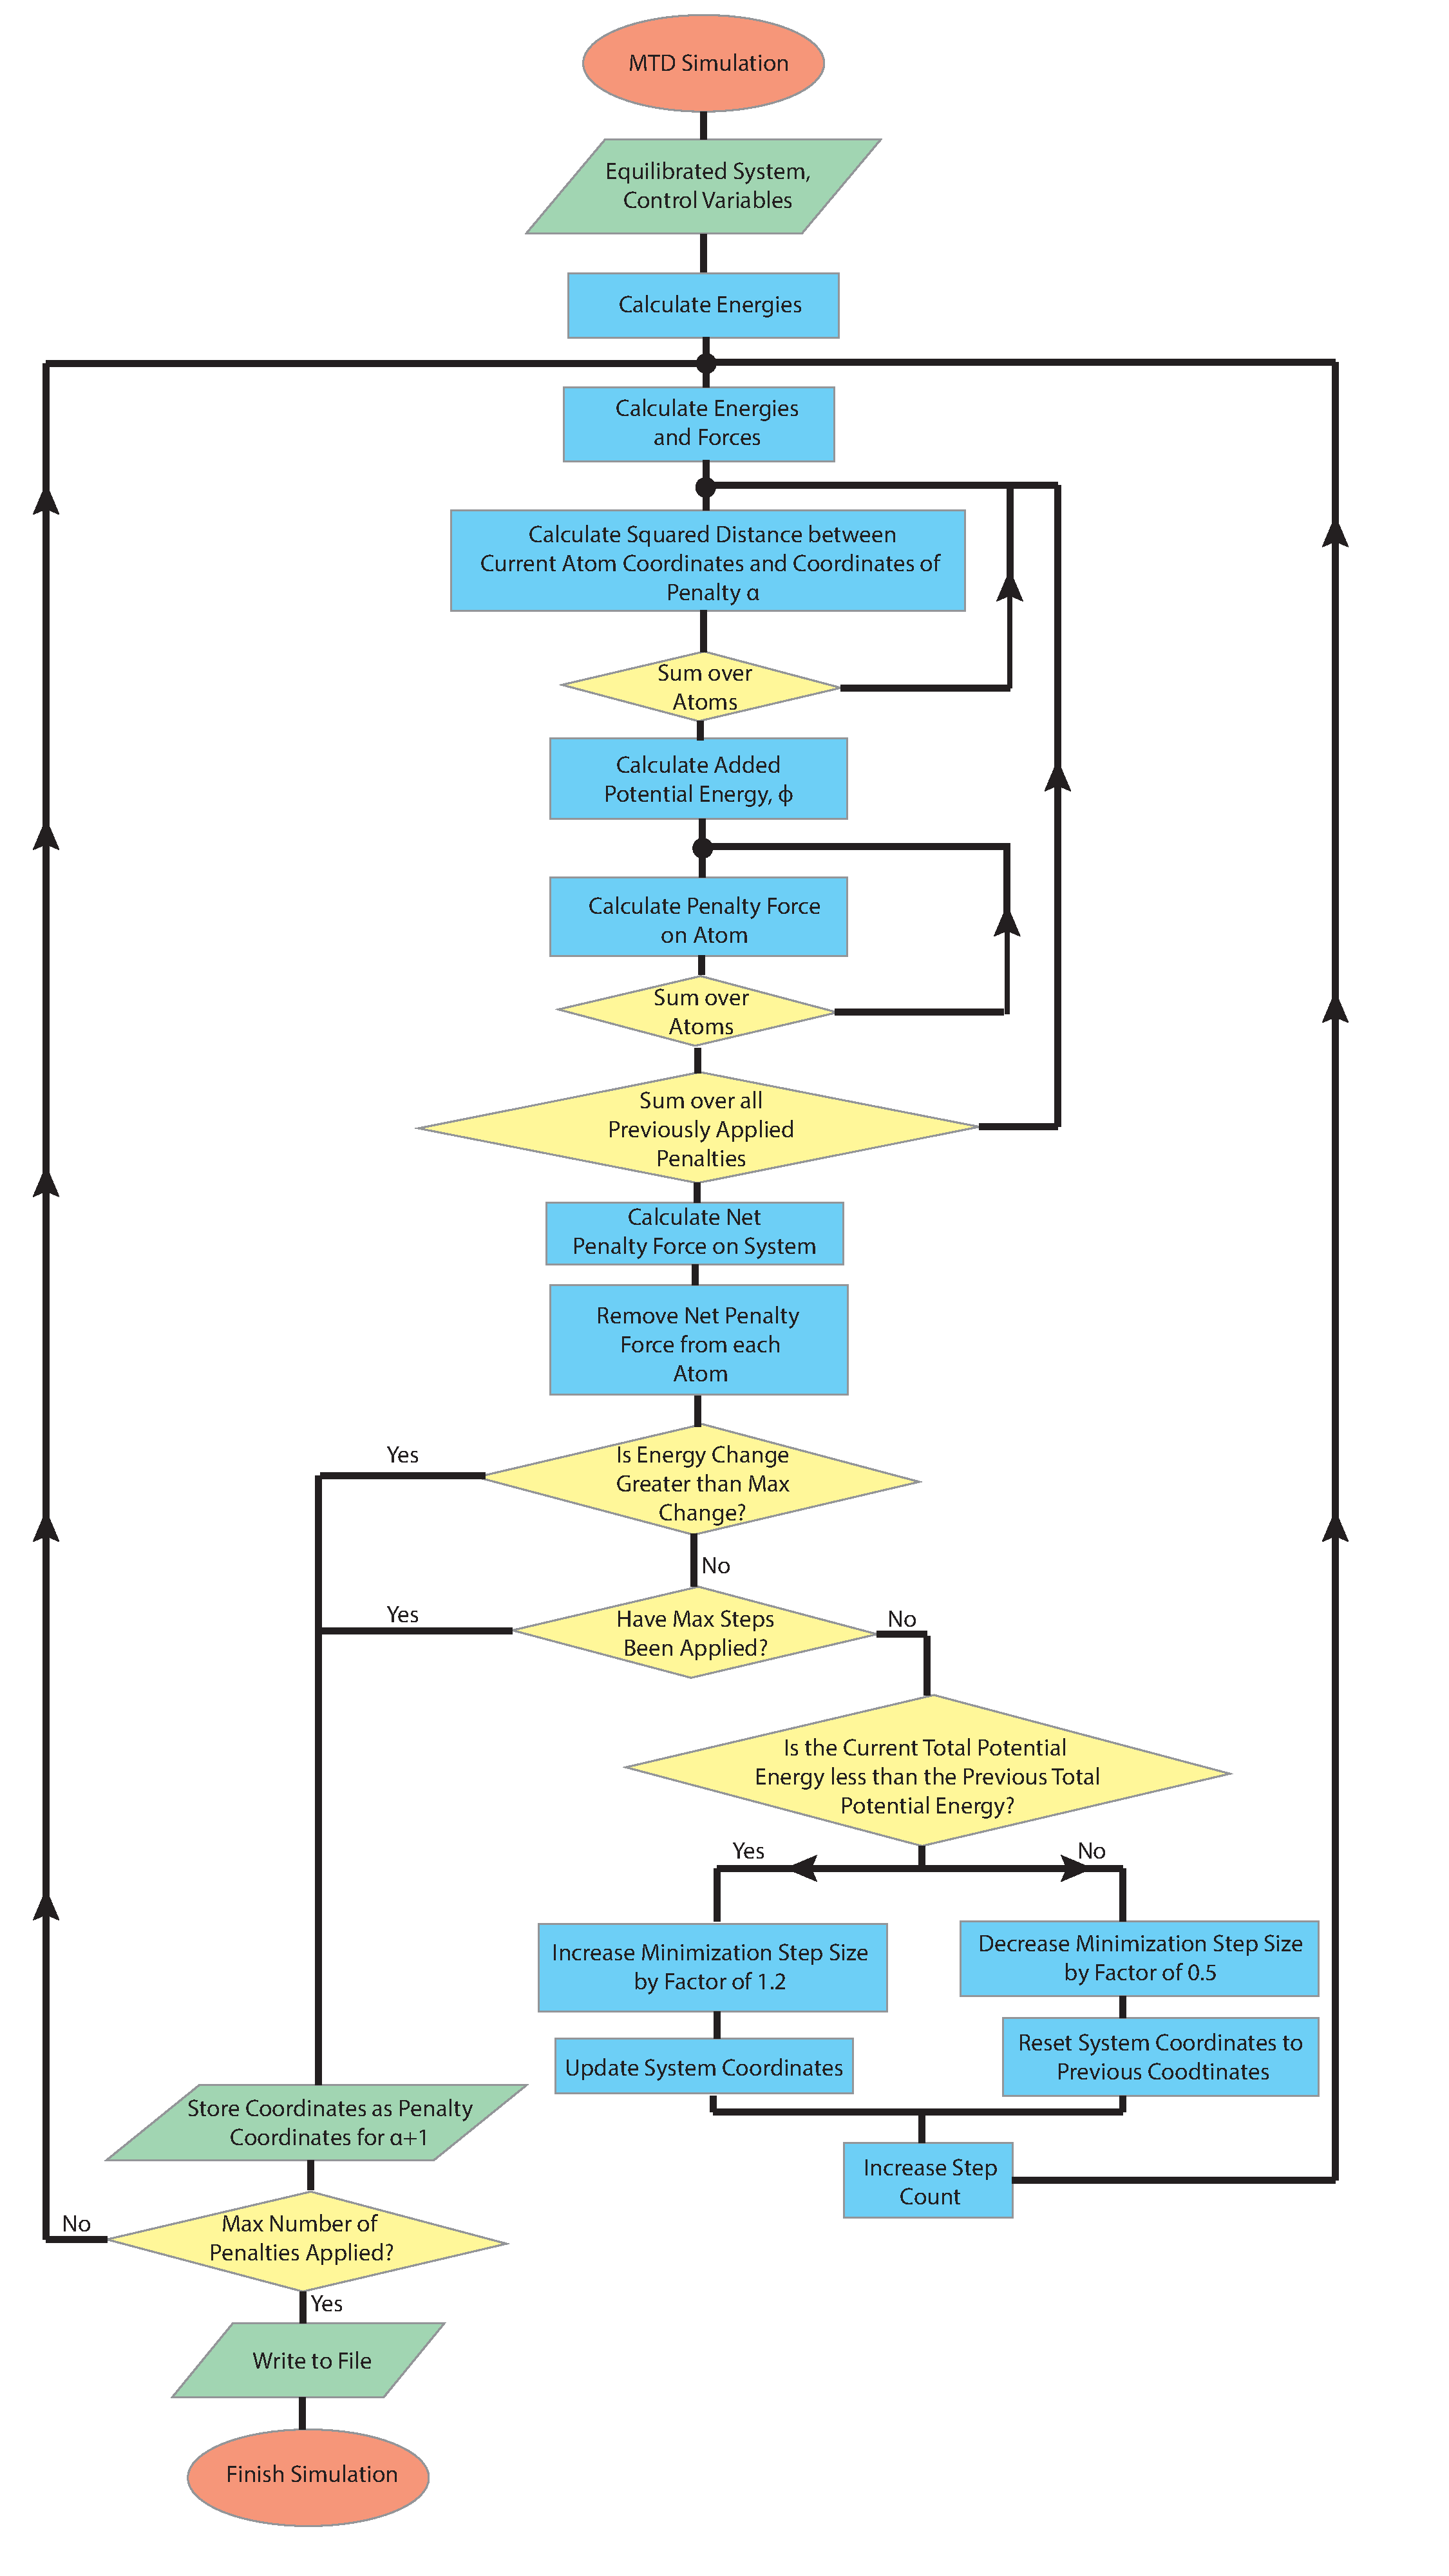
\includegraphics[height=.95\textheight]{./Figures/Appendix/MTD_flowchart.pdf}
	\caption{A schematic flow chart of the metadynamics code implemented into GROMACS.}
	\label{flowchart}
\end{figure}